\section{Backend}
В данном разделе рассмотрены технологии, с которыми пользователь непосредственно
не взаимодействует. Поскольку разрабатываемая нами информационная система
является клиент-серверным веб-приложением, здесь будет рассмотрена так
называемая серверная компонента.

\subsubsection{Ruby}
Создатель Ruby — Юкихиро Мацумото (Matz) — интересовался языками
программирования, ещё будучи студентом, но идея о разработке нового языка
появилась позже. Ruby начал разрабатываться 23 февраля 1993 года и вышел в свет
в 1995 году.

Название навеяно языком Perl, многие особенности синтаксиса и семантики из
которого заимствованы в Ruby: англ. pearl — «жемчужина», ruby — «рубин».

Целью разработки было создание «настоящего объектно-ориентированного», лёгкого в
разработке, интерпретируемого языка программирования.

Язык следует принципу «наименьшей неожиданности»: программа должна вести себя
так, как ожидает программист.

\subsubsection{Ruby on Rails}
Фреймворк Ruby on Rails был создан Давидом Хейнемейером Ханссоном на основе его
работы в компании 37signals над средством управления проектами Basecamp и
выпущен в июле 2004 года.

Ruby on Rails определяет следующие принципы разработки приложений:

\begin{enumerate}
  \item предоставляет механизмы повторного использования, 
позволяющие минимизировать дублирование кода в приложениях (принцип Don’t repeat yourself);
  \item по умолчанию используются соглашения по конфигурации, типичные для
большинства приложений (принцип Convention over configuration).
\end{enumerate}

\subsubsection{Концепция MVC}
Основными компонентами приложений Ruby on Rails являются модель (model),
представление (view) и контроллер (controller). Ruby on Rails использует
REST-стиль построения веб-приложений.

\subparagraph{Модель.} 
Модель предоставляет остальным компонентам приложения объектно-ориентированное
отображение данных (таких как каталог продуктов или список заказов). Объекты
модели могут осуществлять загрузку и сохранение данных в реляционной базе
данных, а также реализуют бизнес-логику.

Как уже говорилось выше, для хранения объектов модели в реляционной СУБД по
умолчанию в Rails 3 использована библиотека ActiveRecord. Конкурирующий аналог —
DataMapper. Существуют плагины для работы с нереляционными базами данных,
например Mongoid для работы с MongoDB.

\subparagraph{Представление.}
Представление создает пользовательский интерфейс с использованием полученных от
контроллера данных. Представление также передает запросы пользователя на
манипуляцию данными в контроллер (как правило, представление не изменяет
непосредственно модель).

В Ruby on Rails представление описывается при помощи шаблонов ERB. Они
представляют собой файлы HTML с дополнительными включениями фрагментов кода Ruby
(Embedded Ruby или ERb). Вывод, сгенерированный встроенным кодом Ruby,
включается в текст шаблона, после чего получившаяся страница HTML возвращается
пользователю. Кроме ERB возможно использовать ещё около 20 шаблонизаторов, в том
числе Haml.

\subparagraph{Контроллер.}
Контроллер в Rails — это набор логики, запускаемой после получения HTTP-запроса
сервером. Контроллер отвечает за вызов методов модели и запускает формирование
представления.

Соответствие url адреса и контроллера задается в файле config/routes.rb.

Контроллером в Ruby on Rails является класс, наследованный от \\
ActionController::Base. Открытые методы контроллера являются так называемыми
действиями (actions). Action часто соответствует отдельному представлению.
Например, по запросу пользователя admin/list будет вызван метод list класса
AdminController и затем использовано представление \\ list.html.erb.

\section{Дополнительные возможости платформы Ruby on Rails}
\subsubsection{Встроенный генератор Rails Generator}
Использование генератора Rails сопровождает разработчика с момента инициализации
нового проекта. Генератор - это скриптовая программа на языке Ruby, которая на
основе полученных входных данных генерирует на основе шаблонов стандартные файлы
исходного кода проекта. Это избавляет разработчика от рутинной работы по
созданию файлов и папок, которые стандартны для всех проектов Rails.
Классический пример использования представлен в листинге
\ref{lst:rails_new_application}  - инициализация нового проекта .

\begin{lstlisting}[language=Bash,caption=Создание
нового приложения,label={lst:rails_new_application}] 
user@host$ rails generate some_application_name
\end{lstlisting}

\subsubsection{Формы ввода данных}
Формы в веб-приложениях – это основной интерфейс для пользовательского ввода.
Однако, обработка форм может достаточно трудоемкой из-за необходимости описывать
элементы форм, правила валидации данных на стороне клиента и сервера. Rails
устраняет эти сложности, предоставляя хелперы для разметки форм. Помимо
стандартных хелперов, существует библиотека simple\_form. Данная библиотека
сокращает время при написании кода веб-формы, а именно - разработчику не нужно
указывать URL-адрес обработчика запроса (при нажатии кнопки submit); не нужно
вручную прописывать HTML-разметку для элемента, отвечающего за отображение и
хранение значения того или иного атрибута - алгоритм simple\_form сам подберет
необходимую разметку на основании типа данных. Кроме того simple\_form сама
преобразует существующую валидацию (реализованную средствами Rails) в валидацию
на стороне клиента (работающую на javascript). Это дает очевидную выгоду -
поскольку ошибки отсекаются на стороне клиента, снижается нагрузка на сетевое
соединение и на обрабатывающий сервер.

\subsubsection{Рассылка  электронной почты}
Action Mailer позволяет отправлять электронные письма из приложения, используя
модель и представления рассыльщика. Таким образом, в Rails электронная почта
используется посредством создание рассыльщиков, наследуемых от
ActionMailer::Base, и находящихся в app/mailers. Эти рассыльщики имеют связанные
представления, которые находятся среди представлений контроллеров в app/views.

Для рассылки почты не требуется приобретение и развертывание собственного
почтового сервера. Достаточно подключить существующий аккаунт в популярных
почтовых серверах (yandex, gmail) в конфигурационных файлах
(config/environments/production.rb) приложения. Веб-сервер будет отсылать
электронные письма подключившись к аккаунту через протокол SMTP.

В режиме разработчика (development) можно настроить имитацию отправки писем для
проверки правильности работы мейлера и тестирования системы в целом. В этом
случае веб-сервер будет сохранять отправляемые письма в виде файлов, в папку
tmp.

\subsubsection{Система контроля версий базы данных}
Поскольку очень часто (как и в нашем случае) разработчики работают в команде,
возникает проблема контроля версий. Причем данный контроль должен выполняться не
только в отношении исходного кода и задач (см. git, github), но и за состоянием
структуры базы данных.

Данная проблема успешно решается с помощью концепции мигрирования БД. Она
заключается в том, что все изменения базы данных делятся на фрагменты -
миграции.

В первых версиях фреймворка Rails разработчик должен был сам назначить имя
миграции. Это часто приводило к коллизиям и приходилось вручную менять и
миграцию и структуру БД.

В более поздних версиях к имени миграции стал добавляться хэш отражающий дату
создания миграции.

C помощью выбранной системы контроля версий разработчики синхронизируют файлы
миграций между собой и рабочим сервером (рис. \ref{ris:development_migrations}).

Active Record отслеживает, какие миграции уже были выполнены, поэтому все, что
нужно сделать, это обновить свой исходный код и запустить rake db:migrate.
Active Record сам определит, какие миграции нужно запустить, проверив таблицу
базы данных schema\_migrations, автоматически создаваемую при изначальном вызове
rake db:migrate. schema\_migrations содержит единственный столбец с именем
versions, содержащий временные метки, с которых начинаются созданные миграции
Active Record (рис. \ref{ris:migration_algorithm}). Каждая временная метка,
содержащаяся в schema\_migrations, показывает, что миграция, связанная с временной меткой, была
вызвана ранее, и не должна быть вызвана при будующих вызовах rake db:migrate. Он
также обновит файл db/schema.rb в соответствии с новой структурой базы данных.

\begin{figure}[h]
\center{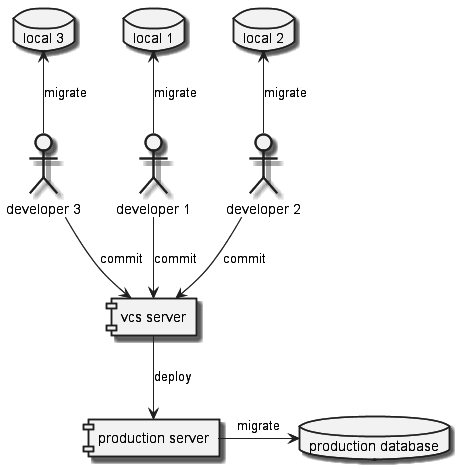
\includegraphics[width=0.5\linewidth]{development_migrations.eps}}
\caption{Централизованный контроль версий базы данных.}
\label{ris:development_migrations}
\end{figure}

\begin{figure}[h]
\center{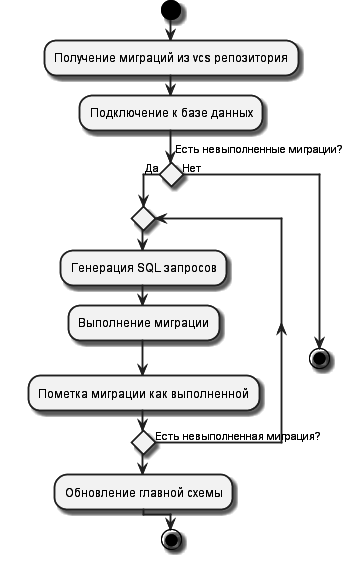
\includegraphics[width=0.5\linewidth]{migration_algorithm.eps}}
\caption{Схема выполнения миграции.}
\label{ris:migration_algorithm}
\end{figure}

\section{Использование сторонних библиотек на языке Ruby}
В процессе разработки проекта для решения многих типовых задач также были
использованы библиотеки из хостинга RubyGems. Как правило для каждой задачи
используется соответствующая библиотека (или группа библиотек). Перечень всех
библиотек находится в файле Gemfile. Для установки библиотек на компьютер
разработчика, а также на рабочую машину системы производится с помощью
специальной утилиты Bundler, которая читает перечень гемов из Gemfile, скачивает
необходимые библиотеки с хостинга и выполняет постинсталляционные скрипты. После
установки всех необходимых библиотек Bundler фиксирует версию каждой библиотеки
в файле Gemfile.lock. Фиксирование версий библиотек позволяет снижать риск
несовместимости между библиотеками при развертывании приложения на рабочем
сервере.

\subsubsection{Аутентификация и авторизация}
Данная задача была самой первой и ее причины очевидны - обработка личной
медицинской информации предполагает тщательной сохранение медицинской тайны.
Разграничение прав доступа к данным и функционалу также крайне необходимы -
недопустимо чтобы доктор мог изменять значения, введенные пациентом. В то же
время некоторые сведения о пациентах и о других пользователях могут быть
изменены (например, фамилия).
Проанализировав эти и другие требования (такие как простота и стоимость
реализации) мы пришли к выводу что для организации функции аутентификации и
аутентификации необходимо использовать стороннюю библиотеку devise, а для
функции авторизации библиотеку CanCan.

\subsubsection{Доступ к базе данных}
Для взаимодействия с хранилищем данных проект на Ruby on Rails использует
специальные библиотеки. Для каждой СУБД существует своя библиотека подключений.
В нашем проекте использует Postgresql 9.1 (подробнее см. ниже). Для подключения
к данной СУБД существует библиотека pg.
    
Среда Rails для манипулирования данными вызывает функции из этой библиотеки,
далее внутри в библиотеки происходит их преобразование в sql и далее запрос
отправляется к СУБД. Данные для подключения библиотека берет из файла
конфигурации.

\subsubsection{Служебная утилита rake}
Rake\footnote{
	\url{http://ru.wikipedia.org/wiki/Rake}
} — инструмент для автоматизации сборки программного кода. Он подобен
SCons, Make и Apache Ant, но имеет несколько отличий. Этот инструмент написан на языке
программирования Ruby. Автором Rake является Jim Weirich.
Rake использует блоки анонимных функций Ruby для определения различных задач,
используя синтаксис Ruby. В нем есть библиотека основных заданий, таких как
функции для задач манипулирования файлами и библиотека для удаления
скомпилированных файлов (задача «очистки»). Как и Make, Rake может также
синтезировать задачи, основываясь на шаблонах (например, автоматическая сборка
задачи компилирования файла на основе шаблонов имен файлов).
При работе с Ruby on Rails утилита rake занимает особое место. С помощью данной
утилиты выполняется много служебных действий как в режиме разработчика, так и на
рабочей машине. С помощью данной утилиты происходит выполнение миграции и запуск
websocket сервера.

\begin{lstlisting}[language=Bash,caption=Выполнение миграций
,label={lst:rails_new_application}] 
user@host$ rake db:migrate
\end{lstlisting}

\begin{lstlisting}[language=Bash,caption=Компиляция ресурсов
,label={lst:rails_new_application}] 
user@host$ rake assets:precompile
\end{lstlisting}
 
 Данная команда запустит процедуру компиляции материалов веб-страниц на рабочей
 машине (см. раздел fronted).
 
 \subsubsection{Тестирование отправки писем}
 Для этого используется библиотека mailcatcher. По сути это простейший
 SMTP-сервер который перехватывает письма и позволяет просматривать их с помощью
 веб-интерфейса.
 
 \section{Postgresql}
Основными критериями при выборе СУБД были: открытость, функциональность и
наличие опыта работы с данной базой данных, а так же простота интеграции с
выбранным стеком технологий. Выбор был сделан в пользу Postgresql.

Для работы с Postgresql для Ruby On Rails существует библиотека pg, реализующая
Active Record Query Interface специфичный для Postgresql.

Данная база данных достаточно надежна и проста в обращении.

Основные преимущества:
\begin{enumerate}
  \item GNU General Public License;
  \item встроенный механизм полнотекстового поиска;
  \item простая реализация резервного копирования базы в реальном времени;
  \item наличие готовых средств для баллансировки нагрузки;
  \item с версии 9.0 поддерживается потоковая репликация (Hot Standby);
  \item транзакционный DDL.
\end{enumerate}

\section{Websocket}
Одной из целью создания системы является - постоянный обмен актуальной
информацией о состоянии пациента.
	
Websocket сервер позволить организовать это взаимодействие в реальном времени с
минимальными задержками, за счет возможности инициировать передачу информации с
backend во frontend на стороне backend.
	
Для работы с Websocket сервером используется одноименный протокол WebSocket\footnote{
	\url{http://ru.wikipedia.org/wiki/WebSocket}
}.

Основной задачей Websocket сервера является оповещение подписчиков о наступлении
определенного события и отправке подписчикам метаданных связанных с событием.
Событием в рамках приложения может быть:
\begin{enumerate}
  \item любая CRUD операция над моделью;
  \item выполнение какого-либо бизнес-процесса.
\end{enumerate}

Реализация Websocket сервера базируется на библиотеке Eventmachine\footnote{
	\url{http://rubyeventmachine.com/}
}. В текущей реализации Websocket сервер позволяет выполнять следующие операции:
\begin{enumerate}
  \item присоединение/отсоединение клиента от определенного канала;
  \item передача сообщений как в рамках определенного канала, так и
широковещательных сообщений.
\end{enumerate}

На стороне клиента используется стандартный объект WebSocket обернутый в класс
на CoffeeScript для более удобной работы.
